% ------------------------
\mysec{Winkel im Bogenmaß}
% ------------------------
\begin{minipage}{0.44\linewidth}
  \centering
  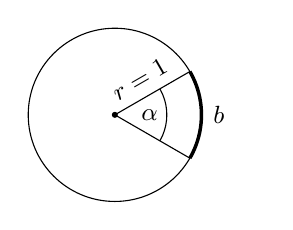
\begin{tikzpicture}[scale=1.1]
    \fill (0, 0) circle (1pt);
    \draw (0, 0) circle (1cm);
    \draw (30:1cm) -- (0, 0) -- (330:1cm);
    \begin{scope}
      \clip (30:2cm) -- (0, 0) -- (330:2cm);
      % Winkel
      \draw (0, 0) circle (6mm);
      % Bogenlaenge
      \draw[line width=1.25pt] (0, 0) circle (1cm);
    \end{scope}
    % Beschriftung
    \node at (0:4mm)  {{\small$\alpha$}};
    \node at (0:12mm) {{\small$b$}};
    \node[rotate=30] at (55:5mm) {{\small$r=1$}};
  \end{tikzpicture}
\end{minipage}%
\begin{minipage}{0.55\linewidth}
  \formrow{\frac{\alpha^{\circ}}{360^{\circ}}=\frac{b}{2\pi}}
  \formrow{\alpha^{\circ}=b\cdot\frac{180^{\circ}}{\pi}}
  \formrow{b=\alpha^{\circ}\cdot\frac{\pi}{180^{\circ}}}
\end{minipage}
